\documentclass{report}
\usepackage{amsmath, amssymb, placeins, url, verbatim}
\usepackage[hyperref,ibidtracker=false,backend=bibtex,hyperref=false]{biblatex}
\usepackage[acronym,description,toc]{glossaries}
\usepackage{titlesec}
\usepackage{emp}
\usepackage{listings,color}
\usepackage{hyperref}
\usepackage[parfill]{parskip}

% Reset acronyms at each chapter
\titleformat{\chapter}[display]
    {\normalfont\huge\bfseries}{\chaptertitlename\ \thechapter}{20pt}{\Huge}[\glsresetall]
    
\ifx\pdftexversion\undefined
\usepackage[dvips]{graphicx}
\else
\usepackage[pdftex]{graphicx}
\DeclareGraphicsRule{*}{mps}{*}{}
\fi

\usepackage{breqn}
\addbibresource{\jobname.bib}
\setcounter{secnumdepth}{3}
\setcounter{tocdepth}{3}
\newcommand{\coststar}{\mathbf{c^*}}
\newcommand{\seeg}{\footnote{See glossary}}

\newenvironment{definition}[1][Definition]{\begin{trivlist}
\item[\hskip \labelsep {\bfseries #1}]}{\end{trivlist}}

\newenvironment{proof}[1][Proof]{\begin{trivlist}
\item[\hskip \labelsep {\bfseries #1}]}{\end{trivlist}}

% Glossaries stuff

% ORM
\loadglsentries{glossary.tex}
% \makeglossaries


\lstset{language=Python,showstringspaces=false,formfeed=\newpage,tabsize=4,commentstyle=\itshape,basicstyle=\ttfamily,morekeywords={lambda, forms},captionpos=b,numbers=left,keywordstyle=\color{blue}}

\title{Djangorifa: A reports-facilities-management bidding system}
\author{Caroline Glassberg-Powell}

\begin{document}
\maketitle

\begin{abstract}
The World Bank Group has been funding development of web applications for developing countries. As the mobile telephony market grows in Africa, more focus is being spent on facilitating the development of public facilities through the mobile web. One of these focuses is a reports management system for citizens to report problems with their town.

There is, however, little focus on what happens to the reports after they are made. There is need for a transparent chain of report-making whereby a citizen makes a report and can track its progress.

I have created a web application through which people can report civic issues and track the report's progress. This project uses data from a slum in Africa to exemplify this idea.
\end{abstract}

\tableofcontents

\chapter{Introduction}
\section{Objective}
The \gls{WBG} is currently funding development projects in Africa. One of the focuses is a centralised reports management system to allow members of the public to report problems with public facilities.

This project aims to create an open-source web application which provides a facilities-reports-management system whereby reports made by citizens can be tracked and managed.

The finished product should be deployable in different countries with minimal configuration, and be easily extensible by other programmers.

\section{Motivation}
This project is motivated by the desire to use the skills gathered during my three years at university to develop a project which is beneficial to people. I was a core member of the winning team at 2011's London Water Hackathon, where I spent 24 hours hacking an existing reports management system, Ushahidi Web~\cite{ushahidiweb}.

This is used primarily in Africa to gather information about currently occurring crises; for example, it was used in the immediate aftermath of the Haitian earthquake.

Ushahidi has many limitation, not least of which that it is being maintained with a deprecated version of Kohana PHP~\cite{kohana}, a web framework. Additionally, it is only applicable for currently occurring problems, there is no follow-up on the reports created.

The civic issue tracker Open311 is used by many cities in the developed world~\cite{open311known} to gather non-urgent reports - FixMyStreet~\cite{fixmystreetuk} is one of the better known implementations - but it is unstable~\cite{open311api}. Once a report has been made, it is sent to the council who are responsible for addressing the problem. If they choose to ignore it, the user does not necessarily receive feedback.

The proposed system aims for a transparent process by facilitating the chain from report-made-on-facility to report-completed. As far as can be discerned, there is no existing product which caters for this.

The target market is councils of developing countries (with the focus on Africa) where there are few, or no, public ICT services. There is therefore a niche for a public facilities manager.

Ushahidi and Open311 are focussed around the web. Over 85\% of internet users in Africa use their mobile phones as a connection point~\cite{africainfo}; although the Internet penetration rate is just 5\%~\cite{africainfo}. Africa also has the fastest growing take-up rate of mobile telephony~\cite{africainfo}.

There is a need for a product which caters to this mobile trend that enables citizens to interact with their local councils.

\subsection{Considerations}
When introduced to the project at the London Water Hackathon, Ushahidi was demonstrated using data from a slum called Tandale in the city of Dar es Saalam, Tanzania. Mark Iliffe~\cite{markiliffe}, the team leader for the project, and others have extensively mapped this area and published the data on OpenStreetMap~\cite{openstreetmap}.

Because there is such extensive data, Tandale will be used as the use-case for the implementation of the project. There is a movement for OpenStreetMap to extend its mapping of Africa~\cite{openstreetmapafrica}, so in the future Tandale will no longer be unusual in this respect.

Bribery and corruption are common in Africa~\cite{corruption}, so any design will be carefully considered to make reporting and the follow-up as transparent as possible to the general public. Preventing nepotism and making the system fair is paramount.

\subsection{Challenges}
A web application has been written in Django - a Python web framework - which has been designed to be pluggable and customisable by a programmer with little skill. The application is named Djangorifa, which is the name of the web application, ``Django", combined with the Swahili for ``reports".

The application consists of a reports management system and a facilities management system.

Performance was a challenge: the technology the application runs off is likely to be old.

This report covers the journey taken in developing the system.
\chapter{Background Research}
\label{sec:br}

There are three types of user considered throughout:
\begin{itemize}
\item Super-administrator: the person who configures the system but is not involved in the day-by-day affairs.
\item Administrator: someone at the council who can control and administer the system.
\item Citizen: a person who is interested in reporting problems with a facility.
\end{itemize}

Djangorifa can be divided into two main components:
\begin{itemize}
\item Reports Management
\item Facilities Management
\end{itemize}

The decisions made for the Reports and Facilities Management are discussed in the relevant implementation section Section~\ref{sec:rm}.

A brief introduction to Django and an explanation for why it was chosen can be found in Section~\ref{br:django}.

\section{Django}
\label{br:django}

My requirements for a web framework were:
\begin{itemize}
\item Written in a language I know.
\item Offers geo-spatial database queries.
\item Detailed documentation and a large community of support.
\end{itemize}

PHP was automatically ruled out. I have used it extensively and do not think it is good enough to build a robust, easily maintained codebase. ~\cite{phpsucks} details very clearly the reasons against PHP.

Two frameworks which fit all the requirements were therefore considered: Ruby on Rails~\cite{rails} and Django~\cite{django}.

I decided to try Ruby on Rails. After two days, I realised it does not have object-oriented forms; HTML forms are defined by strings.

Django has object-oriented forms, and these became necessary. Therefore, I switched to Django.

\section{Introduction to Django}
Django is known as an \gls{MVT} framework. Each component of a web application can be separated into an app, which is a folder\footnote{Which must be in the Python path} containing a ``models.py" file, a ``views.py" file and a ``templates" directory. An app may also declare an ``admin.py" file which Django uses to provide an administration section.

The main directory of the web application contains a ``settings.py" file. This file specifies the database in use and the locations of all the apps in the application.

\subsection{Model}
For an app to store data in the database, classes which subclass ``django.db.models.Model" must be defined in ``models.py". These classes are called models. Each model can define class variables called fields. As an example:

\begin{figure}[thp]
	\centering
	\begin{tabular}{c}
	\begin{lstlisting}[label={lst:model}]
	class ExampleModel(models.Model):
		field1 = models.CharField(max_length=2)
		field2 = models.IntegerField(max_digits=2)
		field3 = models.ForeignKey(ExampleModel2)
	\end{lstlisting}
	\end{tabular}
	\caption{Example models}
\end{figure}

The command-line operation ``syncdb" tells Django to create a database table for each class, and each field variable as a column in that table. An automatically generated column called ``id" is also added to the database when this command is called. Django provides an abstraction layer, an \gls{ORM}, so database operations can be performed by calling methods on the models (Figure~\ref{lst:savemodel}).

\begin{figure}[thp]
	\centering
	\begin{tabular}{c}
	\begin{lstlisting}[label={lst:savemodel}]
	# Create a new instance of an example model
	# and save it to the database
	em = ExampleModel(field1="Moo", field2="Blah")
	em.save()
	
	# Get the data from the database and change it
	em = ExampleModel.objects.get(field1="Moo")
	em.field2 = "Something"
	em.save()
	\end{lstlisting}
	\end{tabular}
	\caption{Manipulating models}
\end{figure}

\subsection{View}
When a user navigates to a page of a Django application, Django's URL dispatcher looks for a file called ``urls.py" in the application directory on the server. This file contains all valid URLs for the website, which can be defined either as hard-coded strings or as \glspl{regex}. Each URL is defined with a function to be called when the user requests it. The function is in an app's ``views.py".

Functions in ``views.py" perform the logic needed to get the content to display to the user. These functions are passed a \emph{request} object. This contains \gls{session} information and any data sent with a \gls{get} or a \gls{post}. The view must then return Django's encapsulation of an \gls{HTTP} response.

The HTTP response takes a string which will be sent to the browser as HTML. To maintain Django's philosophy of \gls{DRY}, this string can be rendered using a Django function, ``render", which takes three compulsory arguments: the request object; the path to a template; and a dictionary of variables to give to the template, which can be any Python object, for example a model or a string.

\subsection{Template}
The template is an HTML file inside the ``templates" directory of an app. This file contains a mixture of HTML and Django's template language. The template language provides minimal functionality so that the variables provided in the dictionary can be presented.

\begin{figure}[thp]
	\centering
	\begin{tabular}{c}
	\begin{lstlisting}[label={lst:views}]
return render(request,
	"example.html", {
		'x':'moo',
		'y':[1,2,3]
	}
)
	\end{lstlisting}
	\end{tabular}
	\caption{Views function}
\end{figure}

Figure~\ref{lst:template} is an example of what might be returned by a views function. The template language uses ``\{\{ \}\}" to represent a variable, and ``\{\% \%\}" to represent a macro.

\begin{figure}[thp]
	\centering
	\begin{tabular}{c}
	\begin{lstlisting}[label={lst:template}]
	Cows say {{ x }}.
	\end{lstlisting}
	\end{tabular}
	\caption{Example.html}
\end{figure}

When the template is rendered with the render function, the macros are executed and the variables filled in with the values in the dictionary. When Figure~\ref{lst:template} is rendered, the HTML produced is "Cows say moo.Cows say moo.Cows say moo."

\subsection{Admin}
Django provides an administration section where apps can register their models to be added, changed and deleted through the website. (Figure~\ref{lst:adminmodel})

\begin{figure}[thp]
	\centering
	\begin{tabular}{c}
	\begin{lstlisting}[label={lst:adminmodel}]
	class ExampleModelAdmin(admin.ModelAdmin):
		# Customise the admin inside this class
		pass
		
	# Register with the admin
	admin.site.register(
		ExampleModel,
		ExampleModelAdmin
	)
	\end{lstlisting}
	\end{tabular}
	\caption{Manipulating models}
\end{figure}

\subsection{Forms}
Django provides a forms module which facilitates the creation of HTML forms. django-crispy is a third-party module which makes this process even easier: a form object is rendered in the template by ``\{\% crispy form \%\}".

There are two classes of forms this project uses: ModelForm and Form. ModelForm creates a form for the model it's given.

\begin{figure}[thp]
	\centering
	\begin{tabular}{c}
	\begin{lstlisting}[label={lst:modelform}]
	class ExampleModelForm(forms.ModelForm):
		extra_field = forms.CharField()

		class Meta:
			model = ExampleModel
	\end{lstlisting}
	\end{tabular}
	\caption{ModelForm}
\end{figure}

When Figure~\ref{lst:modelform} is rendered, it produces an HTML form with three input fields: field1, field2 and extra\_field. When this form is submitted, called .save() on the form will save the model with the user input data to the database.

Form provides this ability to generate forms, but with no save method or model.

Both classes are validated by Django's validation method when the form is submitted. Extra validation can be added to the field declaration in the code.

\subsection{Database}
\label{sec:web:database}

Django ships with GeoDjango which provides functionality for geospatial queries on a database. GeoDjango can be used with Postgresql~\cite{postgresql} and MySQL~\cite{mysql}, but the latter has limitations~\cite{mysqllims}, so Postgresql has been used.
\chapter{Design and Implementation}
Two separate facets of Djangorifa have been developed:
\begin{itemize}
\item Reports Management
\item Facilities Management
\end{itemize}

This chapter will provide an overview of how the components fit together, and detail the shared components of the system.

\section{Overview}
\label{sec:di:ov}

Figure~\ref{fig:di:uml} is the UML Diagram of the overview of the system. There are other apps which have not been shown because they are not required for understanding how the system fits together. They are, however, discussed later. Note that this was created with the command:

\begin{figure}[thp]
	\centering
	\begin{tabular}{c}
	\begin{lstlisting}[label={lst:graph_models},breaklines=true]
	./manage.py graph_models -n -d -g -e -o overview.png reports facilities auth registration users reports taarifa_config sites
	\end{lstlisting}
	\end{tabular}
	\caption{Code to generate overview UML}
\end{figure}

\begin{figure}[h]
\centering
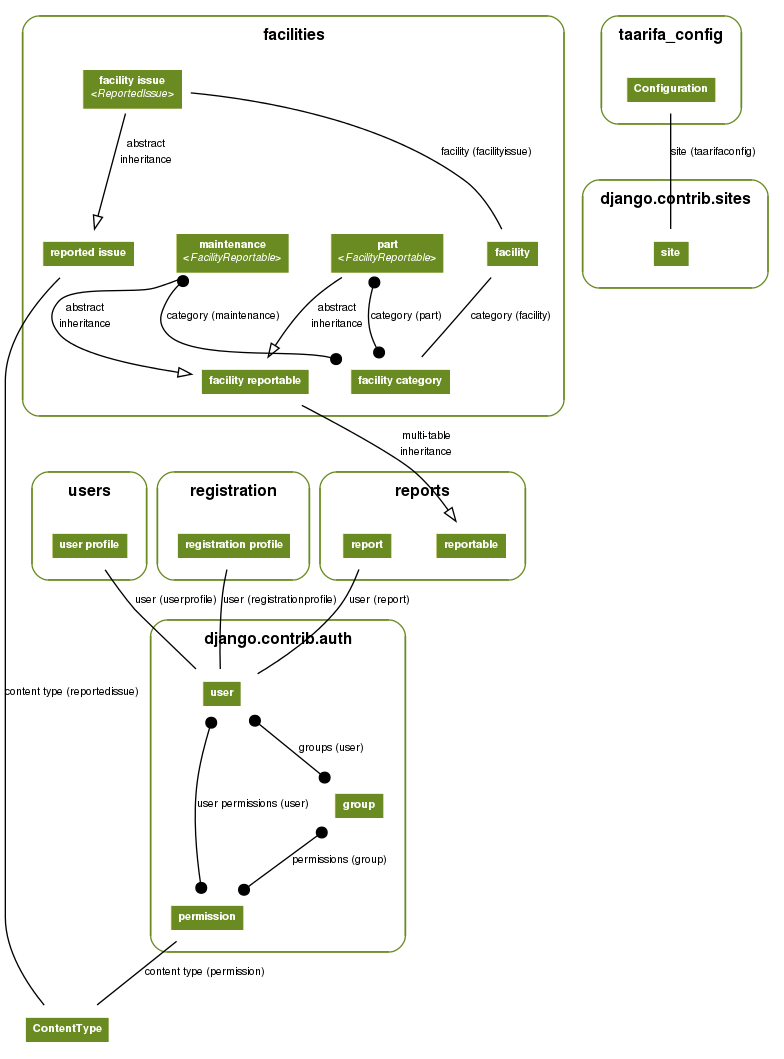
\includegraphics[scale=0.4]{img/overview.png}
\caption{UML Diagram of the overview of the system}
\label{fig:di:uml}
\end{figure}

\FloatBarrier

\subsection{django.contrib.sites}
This is a Django-provided app framework which allows multiple websites to run off the same code. For more information, see \url{https://docs.djangoproject.com/en/dev/ref/contrib/sites/?from=olddocs}.

\subsection{taarifa\_config}
This app was written for an administrator to configure site specific settings. It uses django.contrib.sites to provide different configuration options for different sites using the same database. (Section~\ref{sec:di:admin})

\subsection{facilities}
Facilities management app. Some of its models subclass models provided by reports. (Chapter~\ref{sec:rm})

\subsection{reports}
Reports management app. (Chapter~\ref{sec:rm})

\subsection{registration}
Third-party app called ``django-registration"~\cite{registration} which provides user registration. Parts of it have been overwritten to tailor to Djangorifa. (Section~\ref{sec:di:login})

\subsection{django.contrib.auth}
Django-provided app which provides User, Group and Permission models which are editable through the administration interface. (Section~\ref{sec:di:login}). The ContentType which it points to is an app, django.contrib.contenttypes\footnote{ \url{https://docs.djangoproject.com/en/dev/ref/contrib/contenttypes/}} which is used by Django to keep track of the models in the system.

\subsection{users}
This app was written to provide user profiles so a user can provide additional information about themselves that does not come with django.contrib.auth. (Section~\ref{sec:di:login})

\section{User Registration and Login}
\label{sec:di:login}

Django's default authentication system and django-registration both assume the use of an email address to register, when mobile phones will be the primary method of interaction with the system.

Django.contrib.admin provides:
\begin{itemize}
\item A User model with the required fields: username, password and email address.
\item A Group and Permission model (Section~\ref{sec:di:login:gp})
\end{itemize}

Django-registration provides:
\begin{itemize}
\item Functionality for registering (this is not Django default behaviour)
\item Email address verification
\item Password hashing
\item Password reset
\end{itemize}

It is assumed that users will register with and interact with the system using their mobile phones. Therefore, the registration process had to be changed so as to allow mobile phone number registration.

The users app contains a class called ``MobilePhoneBackend" which is called when a user wants to register. This returns a form ``UserRegistrationForm" when the user views the registration page. The form changes the username field to pass validation only if every character is an integer. The email address field is removed.

When this form is submitted, the email address is saved as the mobile phone number ``@glassberg-powell.com\footnote{My own domain}", for testing purposes. An SMS gateway could be purchased which enables text messages to be sent and received through a website. A few were researched which offered SMS via email. However, they cost money to sign up for, and until the funding is there, the email address will remain as is.

The emails are placed into a task queue by an app called django-mailer~\cite{mailer}. The queue is cleared every 5 minutes by an asynchronous task manager, django-celery~\cite{celery}.

The conceived work-flow is: An SMS will be sent to their phone which they reply to, confirming their phone number.

Django-registration provides an administration interface, but is kept separately from the Django-provided ``User" administration. This is not desired because it separates components which are intrinsically linked. For this reason, the default admin and registration admin interfaces have been disabled, and a custom one written to combine their functionalities.

\subsection{Group and Permission}
\label{sec:di:login:gp}

Groups define groups to which Users can belong. Each Group can have many Permissions which indicate what a User can and cannot do. Every model is automatically created with ``add", ``change" and ``delete" permissions; more can be defined.

Django comes with a super-user and  administrator groups, so ``Citizen" has been defined which provides the permission to make reports. When a user is created, they are automatically added to this group. Permissions to delete or change reports are disabled for transparency reasons. (Appendix~\ref{app:corruption})

\subsection{Profiles}
\label{sec:profiles}

The UML for this app is in Figure~\ref{fig:users}. UserProfile is defined which contains optional details a user may enter about themselves. Future version of Djangorifa might become more of a social network.

\begin{figure}[h]
\centering
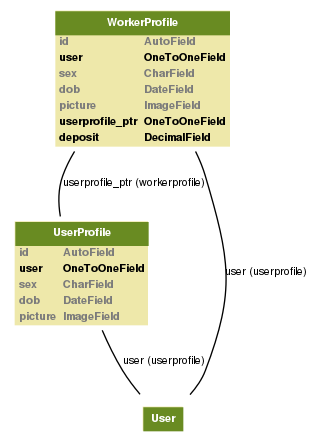
\includegraphics[scale=0.7]{img/users.png}
\caption{Figure to show UML for the users app}
\label{fig:users}
\end{figure}

\section{Administration and Configuration}
\label{sec:di:admin}

\subsection{django.contrib.admin}
An app registers with the admin section through its ``admin.py" file. Classes are defined which allow complete control over the behaviour of models in the admin site.

The admin site automatically creates a view to list all instances of a registered model. If one of these instances is clicked on, the user sees a change form for that instance.

A third-party app called ``django-admin-tools" has been installed which enables in-code overrides of how the administration section appears to the user. The theme is also changed slightly.

\subsection{taarifa\_config}
\begin{figure}
\centering
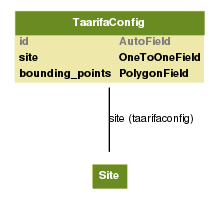
\includegraphics[scale=0.51]{img/config.png}
\caption{UML of taarifa\_config}
\label{fig:taarifa_config}
\end{figure}
An administrator must configure the system on first use. If the system is not configured, they will be forced to the configuration page. Here they will be forced to fill out their user profile (to keep the concept of profiles consistent). They will then be asked to name the site, and to provide the system with the domain name. This is so URL look-up works correctly. They will then be presented with a map where they must draw the bounds of their constituency. This will define where reports and facilities can be defined. There is currently a feature being developed to make a bridge with \gls{OSM}, so this part is currently not 100\% working.

The map is provided by a third-party plugin called ``django-olwidget"~\cite{olwidget}.

An app can implement a model which has a field with a one-to-one relationship with TaarifaConfig (Figure~\ref{fig:taarifa_config}). This model will automatically be displayed on the configuration page, which enables app-specific settings. This is currently not used, but will enable plugins to be developed more easily.

\section{Mobile phone version}
\label{sec:di:mobile}

Django has a middleware framework, which provides an \gls{API} for apps to alter request objects before they are passed to views. django-mobile~\cite{mobile} uses this to add a ``flavour" to each request object, which can either be ``mobile" or ``full". Throughout Djangorifa, if there are separate views for mobile phones, this feature is used.
\chapter{Reports and Facilities Management}
\label{sec:rm}

The use-case for Djangorifa tightly couples the reports management and facilities management. However, as this project may be used solely for reports management, or solely for facilities management, or as a reports-cinema manager, the implementation of reports management is not coupled to facilities.

The reports management has been designed as an interface which can be implemented by apps, to make models reportable.

Currently only a programmer is able to make reportable models, but future versions of the software could enable this to be done through the admin interface.

The facilities management without the reports management is one model which is registered with a slightly customised ModelAdmin.

As such, there is little to say about the facilities management without the reports, so the two are discussed together in this chapter.

\begin{figure}
\centering
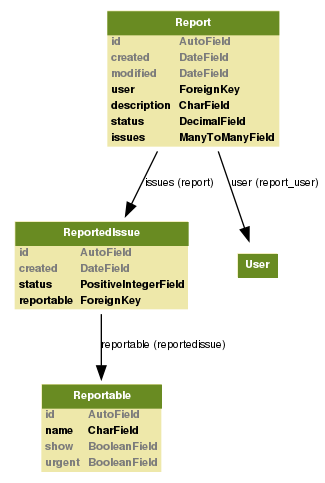
\includegraphics[scale=0.51]{img/reports.png}
\caption{Figure to show UML diagram for the reports management}
\label{fig:rm:uml}
\end{figure}

\FloatBarrier
\section{Reports Interface}
The interface defines two abstract classes and one abstract form class. The UML diagram for the abstract classes is shown in Figure~\ref{fig:rm:uml}; and the class diagram for the form is shown in Figure~\ref{fig:rm:forms}.

To declare an app as reportable, it must have at least two models, one of which subclasses ReportedIssue, and the other Reportable. In order for a user to create a report, the app must contain a form which subclasses ReportForm. A view which contains this form can be presented to the user. On submission of this form, reports are automatically created. All reports created are automatically displayed on the admin page.

The form's default behaviour is to present all Reportables in the system as a list of checkboxes for the user to tick.

\subsection{Reportable}
The Reportable class is an abstract representation for an item in the system which can be reported. For example, a toilet.

As many subclasses of Reportable can be declared as a programmer desires.

\textbf{show} is a boolean to determine whether or not an instance should appear on report forms. When a model instance is deleted through the Django admin, all foreign key relations are also deleted. If a Reportable were able to be deleted, user submitted data would be deleted too. To prevent this from happening, an administrator cannot delete a Reportable once it has been created, they can only toggle its display with this checkbox. This feature has not yet been implemented.

\textbf{Urgent} A boolean which an administrator can use to indicate if a report on the Reportable should be flagged as urgent.

\subsection{ReportedIssue}
A Reportable can be reported many times by different users, but once it is flagged as such, this need only be in the database once. A ReportedIssue is created the first time a report is made for the Reportable.

Only one ReportedIssue can be handled by the report form. No use-case could be conceived where more than one would be required.

\textbf{status} The values in this field are discussed in more detail in Appendix~\ref{app:statuses}. When the status of a ReportedIssue is changed, the user is notified of the change. They can currently toggle notification for all status changes, but in the future they will be able to do this on a per ReportedIssue basis.

Once the status is set to ``Fixed", a ReportedIssue will be created the next time that Reportable is reported.

\subsection{Report}
This class is not designed to be subclassed. One instance is created every time a report form is submitted, storing data of the user who made the report and all the Reportables reported.

\textbf{status} is the percentage of the completed ReportedIssues. This could be calculated on a per-request basis to save the extra work which recalculates the value when the status of a ReportedIssue changes. It was decided that a user might check the status more often than it changes, so calculating the value and storing it may slightly improve efficiency. Otherwise, each time a user wishes to know the status of a report, the Many-to-Many issues field would have to be traversed.
\paragraph{description} Any additional information the user wishes to add.

\subsection{ReportForm}
\label{sec:rm:reportform}

\begin{figure}
\centering
\includegraphics{uml/reports-forms.1}
\caption{Interface diagram for reports management forms}
\label{fig:rm:forms}
\end{figure}

\begin{figure}
\centering
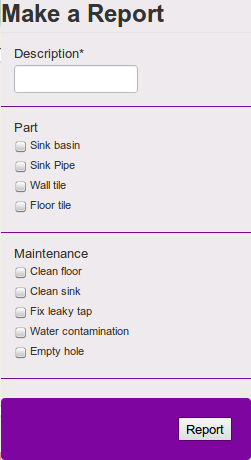
\includegraphics[scale=0.4]{img/reportform.png}
\caption{Example of an implemented ReportForm}
\label{fig:rm:reportform}
\end{figure}

For an app to display a ReportForm which automatically generates the checkboxes of Reportables specific to that report, it can subclass this form.

\textbf{action} is the form action: the URL to which the form is posted.

\textbf{reportables} is a list of all Reportables to be displayed as checkboxes on the form. This defaults to the immediate subclasses of Reportable. Every instance of the model will be rendered as one checkbox, under the title of the Reportable. In Figure~\ref{fig:rm:reportform}, the Reportables are ``Part" and ``Maintenance", and the instances are the checkboxes.

\paragraph{reported\_issue} is the subclass of ReportedIssue which has been implemented.

\textbf{extra\_reportable\_args} are extra arguments which can be provided to the query which retrieves Reportables from the database.

\textbf{get\_extra\_create\_args} If this method is not implemented, a NotImplementedError is raised. When a report has is being saved, a database call is made to see if there are existing ReportedIssues for a given Reportable. A Reportable may be associated with more than one object. For example, 450 facilities have one Reportable toilet. There only need be one toilet which the 450 facilities point to. Therefore, the id of the Reportable is not enough to check the database for existing ReportedIssues, and additional arguments must be provided. The function is given the Reportable currently being saved.

\textbf{clean\_reportable} is an optional function which is called when ReportForm is being validated. It is passed the class of the Reportable being validated, and a list of all checkboxes. This could be used, for example, to prevent two Reportable instances from being reported together.

\section{Facilities Management}
The facilities management implements the interface discussed in the previous section to allow facilities to be reported. The table of user requirements is shown in Table~\ref{tab:rm:fac:req} and the UML for the app is in Figure~\ref{fig:rm:fac:uml}.

\begin{figure}[thp]
\centering
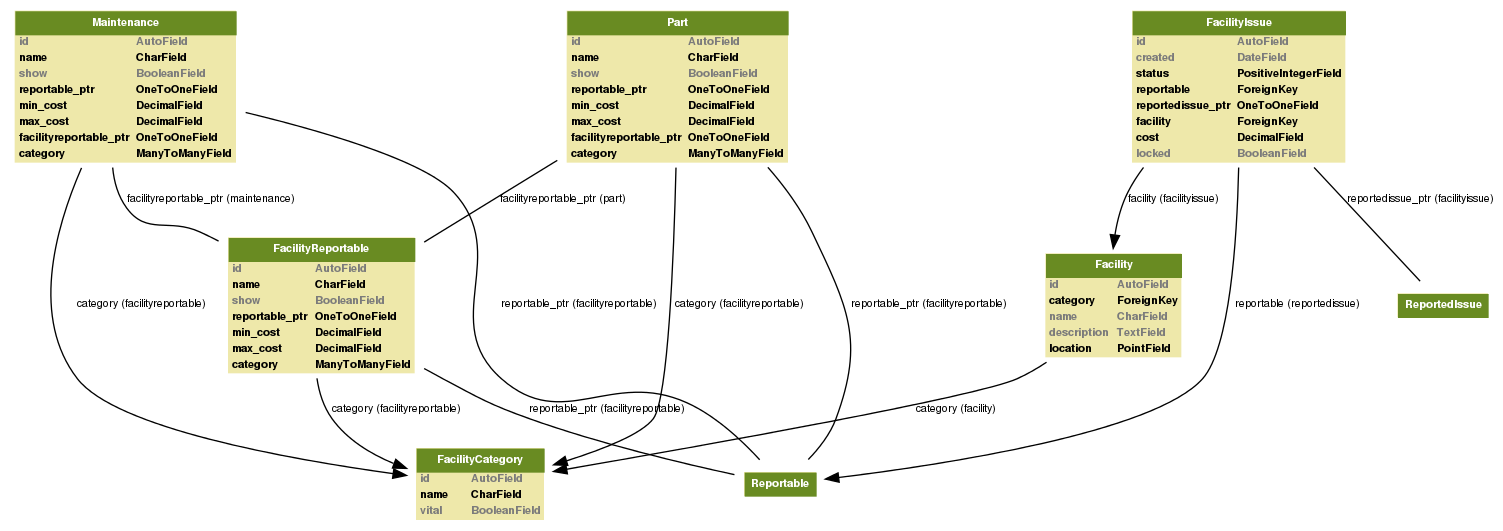
\includegraphics[scale=0.35,angle=90]{img/facilities.png}
\caption{UML diagram for the facilities management}
\label{fig:rm:fac:uml}
\end{figure}

\subsection{User Requirements}
\begin{table}[h]
\centering
\begin{tabular}{p{2.9cm}p{4.1cm}p{4.1cm}}
\textbf{As a...} & \textbf{I want to...} & \textbf{because...} \\
\hline
Administrator & Add, change and delete facilities & I want full control over the facilities \\
\hline
Administrator & Add, change and delete parts for each facility & I want to specify a parts list \\
\hline
Administrator & Add, change and delete services for each facility & Some problems are not parts, and they require service. \\
\hline
Administrator & View reports made on each facility & I want to keep an eye on citizen happiness \\
\hline
Administrator & Change the status of issues & I want to control the system \\
\hline
Citizen & Report a facility problem on my phone or with a website & I'm unsatisfied with something in my town \\
\hline
Citizen & See the status of the reports I have made & Be updated on the happenings of the town \\
\hline
Citizen & Provide feedback on how the report was handled & I believe in customer service \\
\hline
Citizen & See a map of reports in my area & Someone may have already reported the problem I care about \\
\end{tabular}
\caption{Table to show user requirements for the facilities management system}
\label{tab:rm:fac:req}
\end{table}

\subsection{Facility}
The data in Djangorifa was exported from \gls{OSM}~\cite{openstreetmap}, who are currently collating geographical data in Africa~\cite{openstreetmapafrica}. As such, it was decided to model the Facility class on the data exported from \gls{OSM}.

\textbf{location} is a GeoDjango PointField, which enables geo-spatial queries to be performed on the facilities.

\subsection{FacilityCategory} Every Facility is categorised, and in this implementation, there are two categories: ``toilets" and ``drinking\_water" (taken directly from \gls{OSM}).

\textbf{vital} was added when it was decided the urgency of reports could not be handled automatically. If a report is made which is not marked urgent, but does come from a Facility which is vital, it may be more important.

\subsection{FacilityReportable}
This is the class which subclasses Reportable. For facilities management, it was decided to have a Parts list and a Maintenance list.

The Parts list is a way for an administrator to keep stock of the Parts in the facility. In the future, this could be connected to local businesses for stock-ordering.

A Maintenance list is a list of maintenances which may need to be performed. Part and Maintenance are identical classes and are both Reportable. As such, they inherit from FacilityReportable which is abstract.

\textbf{cost} is the estimated cost to service a broken part or to perform a maintenance.

It was decided that Facilities of the same FacilityCategory would have the same parts, give or take one or two. This is why FacilityReportables has a relationship to FacilityCategory and not Facility.

\subsection{FacilityIssue}
FacilityIssue subclasses ReportedIssue.

\textbf{cost} is automatically filled in with the cost of the FacilityReportable when an issue is created (by implementing get\_extra\_create\_args). However, an administrator may decide that they wish to overwrite this field when the issue is reported.

\textbf{locked} is to prevent a read-update race condition happening when updating the cost. This field is specifically implemented for use by the auctions app (no longer in use).

\subsection{Facility ReportForm}
This was an implementation of the ReportForm. As an example of how straightforward it is, the entire class is 16 lines of code.

\subsection{Implementation}
\subsubsection{Admin}
A script has been written to read data in an \gls{OSM} .osm file and convert it into Facility objects. This can be accessed through the administration section.

When adding a facility, the system checks to see if it's within the bounds defined by the administrator. If not, the facility cannot be saved. Originally these bounds were also displayed, but it looked bad and was tricky to implement without breaking. It is assumed that the administrator knows the bounds of his own site. For multiple sites using the same database, the ``current site" will have to be toggled to add facilities. This is not a use-case anticipated to happen often.

All reports made can be viewed through the administration section. The reports are read-only.

Facility is registered through the admin, and django-olwidget~\cite{olwidget} is used to present the facilities on a map. An administrator can click the facilities and be taken to the editing page. Facilities cannot be deleted through the interface because this would delete past data.

The administrator has full control over the Parts and Maintenances, apart from deleting.

An administrator can view all the currently open reported issues with the facility. If the boolean for locked is not set, they are able to change the price of the issue. If the lock is on, an auction is in place and they can no longer do this (again, not in use).

The administrator can only change the status of a job from ``Dispute Resolution" to ``Complete". This is because the jobs system handles the issues' status automatically.

\subsubsection{Citizen}
When the status of a report changes, the citizen is automatically sent an SMS (implemented through a non-existent SMS gateway).

The vision for a user in Tandale using this system is they will be sat on the loo, or squatting over the hole, and a pipe will burst. They pull out their phone, go to the website and report a problem straight away. They do not want to register or login.

The mobile version of the site uses HTML5 browser geolocation to determine where the user currently is. This is automatically sent to the server, which retrieves the report form for the nearest facility to that location. Therefore, the first thing a mobile user will see is a report form (this is sporadic and therefore wasn't testable when implementing).

To submit this form, they do not need to register: an account will automatically be created for them and verification sent to their mobile phone.

The website version's homepage is a large map with click-able facilities. When clicked, a report form tailored to that facility appears (Figure~\ref{fig:rm:fac:home}). To submit the form, a user must register manually with their mobile phone, and return the verification code.

\begin{figure}
\centering
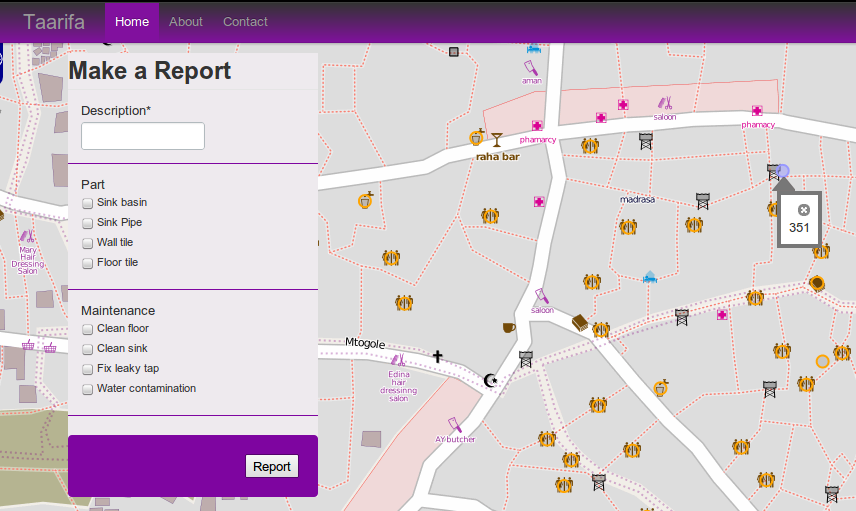
\includegraphics[scale=0.4]{img/home.png}
\caption{Truncated view of the home page}
\label{fig:rm:fac:home}
\end{figure}

\FloatBarrier
\section{Performance}
\label{sec:rm:fac:perf}

There are Many-To-Many relations defined throughout the classes, and these may cause performance issues. The bottleneck when creating a report would occur when the system is checking for existing ReportedIssues.

A script was written to generate a report, and then delete the report 10,000 times, and the total time recorded for each creation, and then averaged.

Originally, this was run with each issue created treated as a separate database call. The average time taken to create a report was 0.3182691201s.

Wrapping the script in a transaction decorator, which sends a transaction to the database, this time was reduced to 0.1430310377s on average.

The same process was repeated without deleting the reports, so 10,000 reports were added to the system. The time taken was 0.1488591671.

Therefore, there is no bottleneck when there are many reports in the system.
\chapter{Conclusions and Future Work}

I have successfully demonstrated that it is possible to build a reports-jobs-facilities management system which is pluggable by a programmer. \\

The initial aim of the project was not to be pluggable by anyone, and it was assumed that someone with a working knowledge of Django would be able to alter the system. However, the project has evolved towards the point where it would be easy to rewrite sections of the code which would enable an administrator to, for example, make a model which was Reportable. \\

As it stands, the system can be installed and run. All that is required is for an administrator to configure the site to the area they have jurisdiction over, input some facility data, and watch the reports come in. \\

I have implemented an algorithm which calculates the best strategy for a ``reverse Dutch" auction for the government. \\

I was unable to find a solution for calculating the urgency of a report based on subjective, qualitative data.

\section{Environmental and Ethical Impact}
I hope that by having this system in place, it will have a positive impact on the local environment. Having been to developing countries and seen the problems caused by faulty sanitation facilities, I hope that a system like this could encourage people to pro-actively change their situation. \\

As hard as I tried to put in safe-guards against this from occurring, the system is still vulnerable to abuse. For example, although workers are unable to bid for jobs, they are more than capable of getting another mobile phone to bid for work. \\

Transparency with persistent data has been strived for, but there's nothing to prevent an administrator from using the command line to delete all data; unless the person who set up the database set-up write-only permissions. \\

If the system is used correctly, I think that it could have a positive impact on local communities.

\section{Lessons learnt}
The biggest lesson I learnt from this project was that as a software engineer, learning when to automate and when not to automate makes the difference in whether or not a system will get used. I think that had I implemented an automated scheduling algorithm, there would have been little chance of a high up-take; mostly because people don't like computers controlling their lives. I really learned how computers are a tool, and like a good carpenter, one should know when and how to use them. \\

When someone was proof-reading my report a while ago, they mentioned that I had a tendency to think from the computer's perspective, rather than from the user's perspective. With that in mind, I really had to try to put myself into an administrator's head. They don't want to fill in lots of boxes or lots of forms to configure the system. \\

From a technical perspective, I learnt a lot about how Django works. The developers believe in the virtue of reading source code to understand how software works; and so it has been instilled into me that Google is the last resort, not the first! \\

This project was mostly about design: my whiteboard was covered in class diagrams for a good few months. As soon as the design was properly formulated, the implementation was fairly straightforward. I also adhered to test-driven development for the most part, testing bits of code that didn't rely on the way Django worked. \\

If I could do it all again, I would spend much less time on the automatic urgency of reports: it simply doesn't need to be automatic. This implementation is much simpler, and it allows an administrator full control over how reports are turned into jobs. I would spend more time developing the auctions app, and thereby be more on the way to integrating money. \\

I would have given myself more than 2 weeks to understand the Optimal Dutch auction. I spent so long trying to work out what the actual algorithm they describe is. I even had email correspondence with one of the authors to try to understand. Most of my time reading the paper was spent scrolling up and time, and everything in the auctions section has been compiled from that arduous process.

\section{Future Implementations}
I plan to take this project as far forward as I can. There are many things I would like to add. Some of these have already been mentioned in the text. The priority is integrated mobile money: as soon as workers have a real incentive to sign up to the system, this product has a big chance to be a success. \\

I would like an administrator to have the ability to dynamically add models through the interface. That way they could declare their own reportable classes without relying on a programmer. On a similar principle, they could declare auctions through the administrative interface.
\appendix

\chapter{Preventing Corruption}
~\label{app:corruption}

In a continent as rife with population as Africa~\cite{corruption}, it is important to ensure that software is open to as little abuse as possible. The suggested method of doing so is by ensuring that all governmental actions are transparent to the public~\cite{transparency}. This means, for a site such as Taarifa, that an administrator cannot delete any information which the public has submitted. \\

Spam may be a problem; but transparency is more important.

\chapter{Statuses}
\label{app:statuses}

There are 5 values the status can take: ``Awaiting verification", ``Awaiting assignment", ``Assigned", ``Fixed" and ``Dispute resolution". For each report which enters the system, an administrator has to verify it. This concept is carried over from the Water Hackathon: this was one of the things I implemented on Ushahidi. \\

The awaiting assignment is awaiting a worker to bid for the job. Assigned and fixed are their namesakes. Dispute resolution is when a citizen has reported that their report has not been handled correctly. The report is then placed into dispute resolution, and the worker's deposit held. Once the issue is sorted, the worker will receive their money back, and the report will go back to complete.
\printglossaries
\printbibliography

\end{document}
